\chapter{Data Generation}
\label{chap:DataGeneration}
\par\noindent
\textit{\textbf{Introduction}} The implemented model may now be utilized to simulate braking processes, generating output data describing the behavior of the train during the process. 

\section{Simulation}
\label{sec:Simulation}
\par\noindent
To recapitulate: We have defined a theoretical model for a train's braking process in chapter \ref{chap:FundamentalsOfRailwayVehicleEngineering}, and implemented this model in simulink in chapter \ref{chap:ModelingOfTrainOperations}. The aim of this work, however, is not only building a model, but also generating a data set describing the train's behavior during its phases of breaking. We can utilize simulink to run a large number of simulations with varying combinations of input parameters. Each simulation represents one train ride, each ride consisting of multiple phases of accelerating, braking and keeping velocity. 

\begin{figure}[H]
	\centering
	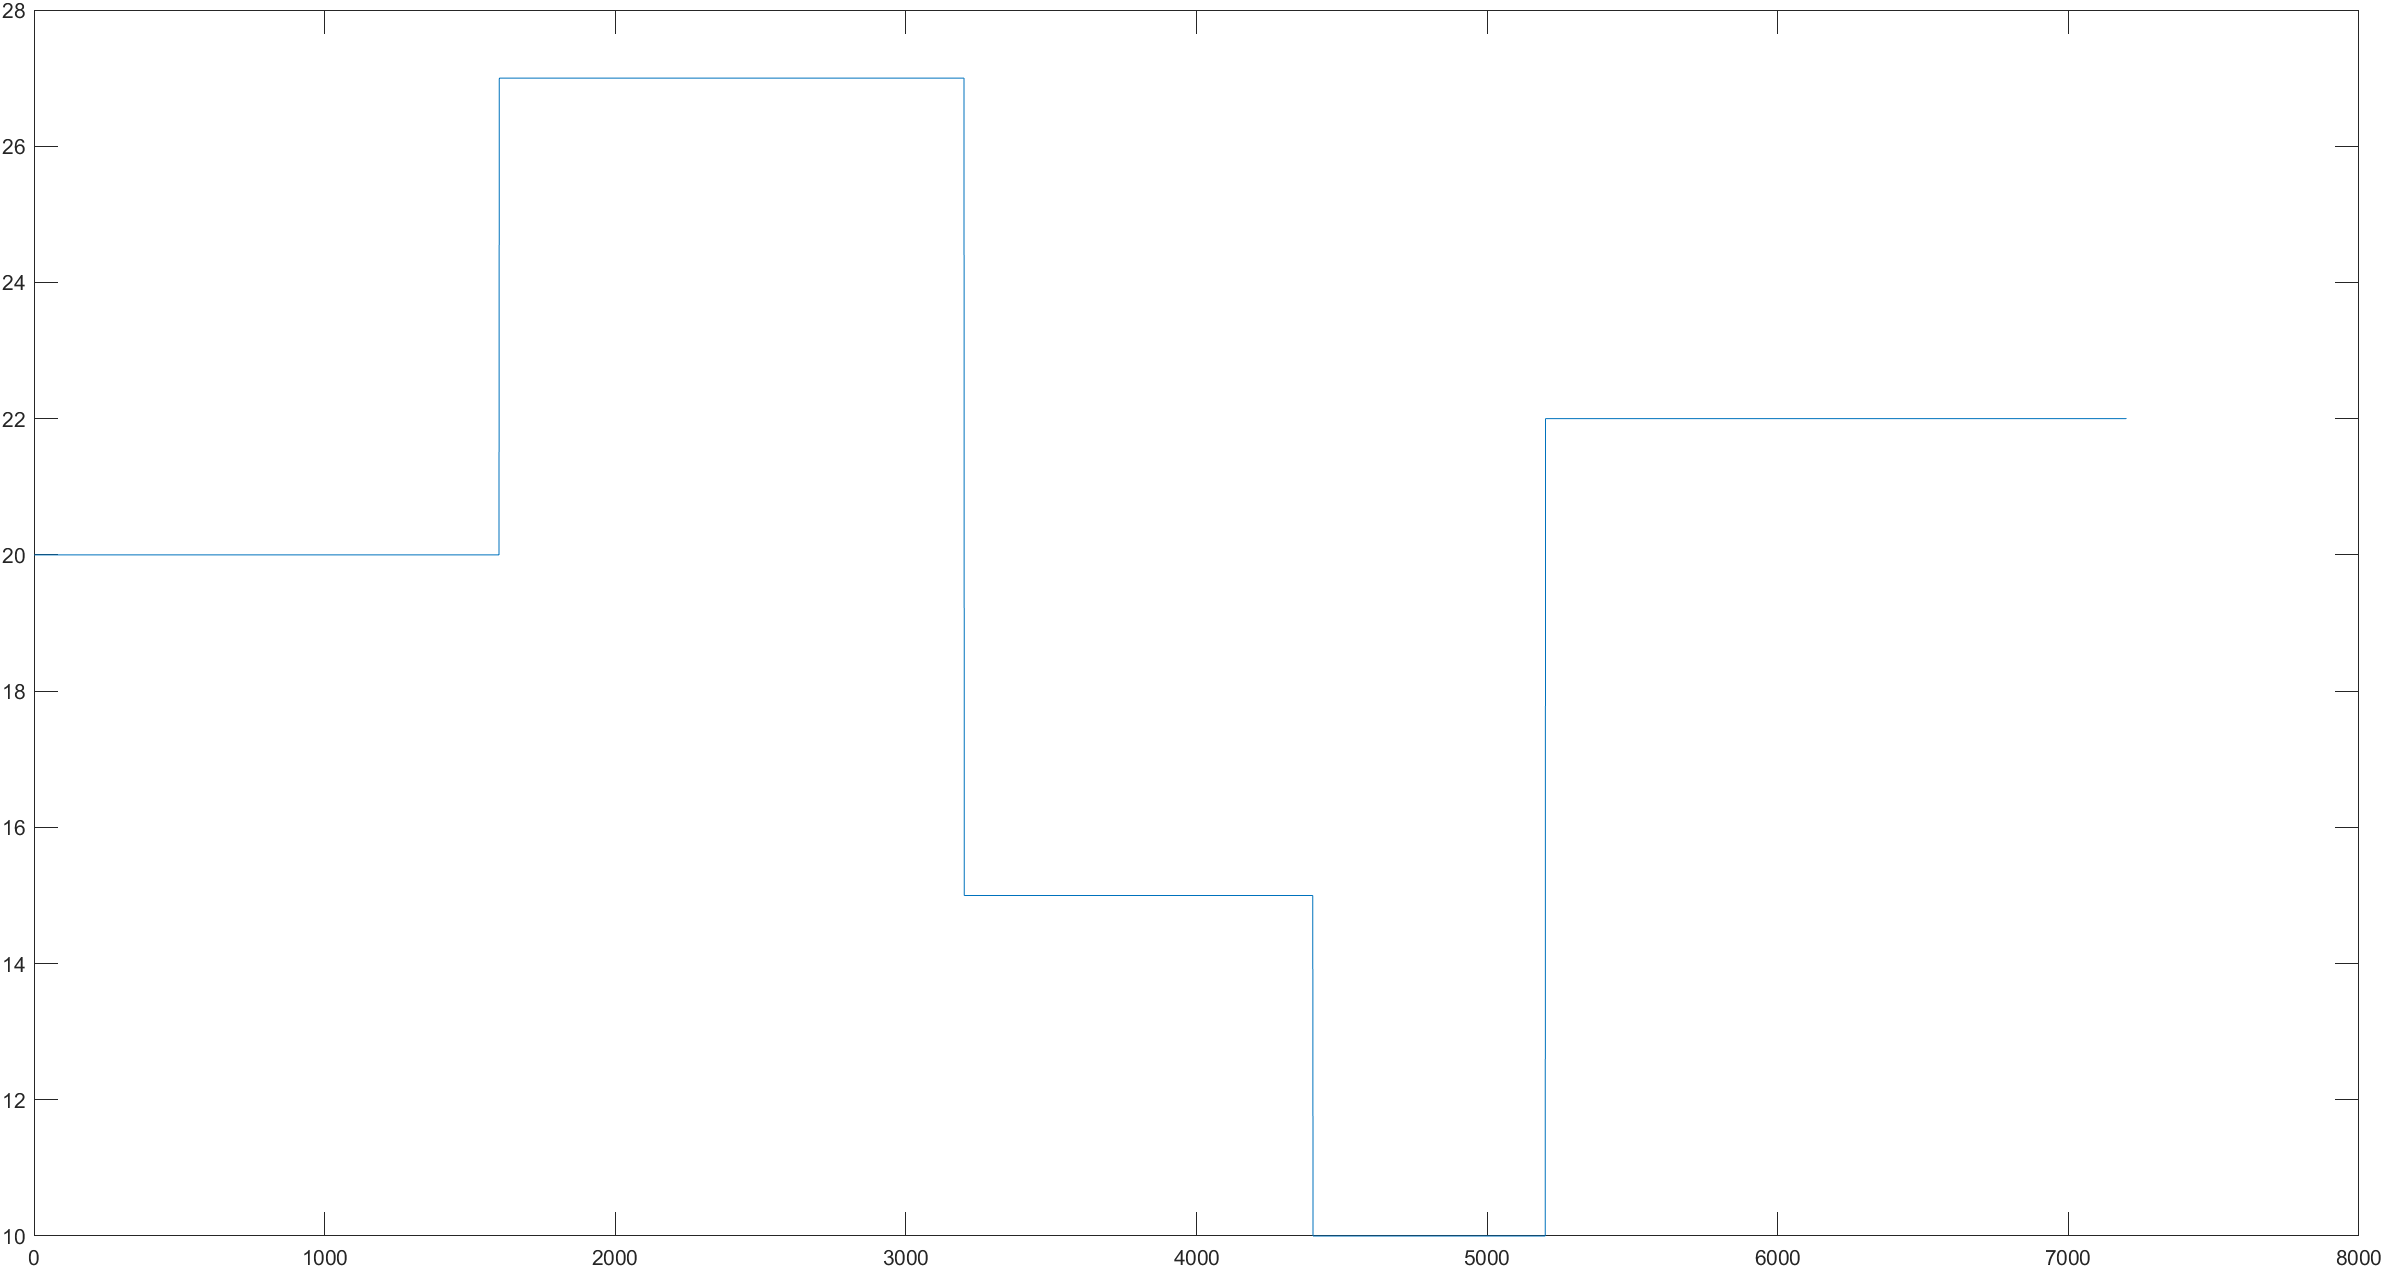
\includegraphics[width=\linewidth]{./pic/input}
	\caption{Simulation Input}
	\label{fig:siminput}
\end{figure}

\par\noindent
Figure \ref{fig:siminput} visualizes how a track profile might look like. It stipulates the maximum allowed velocity for discrete points in time, as well as the overall duration of the simulation; the train either brakes or accelerates accordingly in order to match the corresponding value. An example: Let the simulation time be 1200 seconds, and $v_{max}(1200)=20 \; \frac{m}{s}$. Let the train's velocity $v$ be $25 \; \frac{m}{s}$. The train will engage its brakes (or continue braking, if they have already been engaged) in order to bring $v$ down to $20 \; \frac{m}{s}$. If $v$ were $15 \; \frac{m}{s}$, the train would accelerate instead. The track profile is one of many input parameters, all of which determine the course of the simulation. 

\section{Matlab Code}
\label{sec:MatlabCode}
\par\noindent
A matlab script is used to configure the simulation input, execute the simulation, and write the simulation output into a tabulator-separated file. At the start of execution, the workspace (where variables are stored) should be cleared. Also, the number of cores to use for parallel processing must be set (more on this later):

\bigskip
\begin{python}
clear all
clc
warning ('off','all');
numcores = 10;
\end{python}
\bigskip

\noindent
Generally speaking, simulation input can be divided into two categories: static and dynamic parameters. They, for the most part, correspond to the constants and variables defined in chapter \ref{chap:FundamentalsOfRailwayVehicleEngineering}. The static parameters, i.e. constants, remain the same for every single simulation run, while the dynamic parameters, i.e. variables, may be different for any two simulation runs.

\bigskip
\begin{python}
RBD = 5; 
VBD = 3.5; 
l = 18; 
c = 250; 
\end{python}
\bigskip

\noindent
These constants all correspond to the brake pipe ${\mathcal{M}}_{bp}$, where $RBD$ is the regular operations pressure (i.e. the pressure on the brake pipe when brakes are disengaged), $VBD$ is the full breaking pressure (i.e. the pressure on the brake pipe when brakes are fully engaged), $l$ is the physical length of the brake pipe $l_{bp}$ (although $l_{bp}$ is defined as a variable in ${\mathcal{M}}_{bp}$, it is assumed all wagons have the same physical length for the sake of simplicity), and $c$ is the propagation velocity of the pipe's medium $v_{bp}$.

\bigskip
\begin{python}
tf = 4;
tl = .1;
\end{python}
\bigskip

\noindent
\TODO{}

\bigskip
\begin{python}
p0 = 0;
Pres = 0/1000*[5.7/771 0 1.6];
alpha = 0.9;
BPnum = [0.3 alpha];
BPden = [1 alpha];
\end{python}
\bigskip

\noindent
\TODO{}
\par\noindent
All static parameters have now been initialized. They, along with the track profile, will remain unchanged for all simulations; what sets any two simulations apart is their variable input parameters.

\bigskip
\begin{python}
tmax = 3600;
nmax = tmax * 2;
t = linspace(0, tmax, nmax);
u = [10*ones(1000*2,1); 15*ones(500*2,1); 25*ones(1200*2,1); 12*ones(600*2,1); 0*ones(300*2,1)];
simin.time = t;
simin.signals.values = u;

trackgradient = 0;
\end{python}
\bigskip

\noindent
The code above shows the definition of the track profile. \pyth{tmax} specifies the duration of the simulation in seconds, so in this case one hour. \pyth{nmax} is number of discrete data points; with \pyth{nmax = tmax * 2}, there are on average two data points for every one second of simulation time. \pyth{t} is a linearly spaced vector, i.e. a vector of \pyth{nmax} evenly spaced points between 0 and \pyth{tmax}, which is then set as time input using \pyth{simin.time = t;}. \pyth{u} is the vector which holds the data points, with the number of data points being equal to the value of \pyth{nmax}. The data points stipulate the maximum allowed velocity $v_{max}$ for every discrete point in time. For example, \pyth{10*ones(1000*2,1);} means that for the first 2000 points in time, or for the first 1000 seconds of simulation time, the value of $v_{max}$ is $10 \; \frac{m}{s}$. Continuing with the above example, $v_{max}$ then increases to $15 \; \frac{m}{s}$ for the next 1000 points in time, or the next 500 seconds of simulation time. This vector \pyth{u} is then set as input signal using \pyth{simin.signals.values = u;}. Finally, \pyth{trackgradient = 0;} specifies the average gradient of the track (in this case, the track neither goes uphill, nor downhill).
\par
The goal is to create large quantities of data, i.e. at least hundreds of gigabytes. Since one single simulation run takes, on average, five seconds to complete, and one simulation run produces approximately one megabyte of output data, producing 500 gigabytes worth of data would take 2,500,000 seconds, or almost 29 days. Obviously, this is not acceptable. Fortunately, simulink simulations may be run in parallel, where hardware is the limiting factor rather than time. Albeit, simulations are very expensive, and one will quickly run out of memory if too many simulations are run simultaneously (Using 20 cores, i.e. running 20 simulation in parallel, lead to the server freezing up). Using too many cores also lead to the matlab engine timing out, though whether this was due to memory restrictions or limitations of the engine is unclear. Anyway, using ten CPU cores for parallel processing proved to be stable.

\bigskip
\begin{python}
wagons = 1:1:40;
friction = 0.05:0.01:0.78;
tracforce = 200000:1000:400000;
\end{python}
\bigskip

\noindent
The remaining elements of $\{{\mathcal{V}}\}$ left to address are wagon mass $m$, train composition $comp$, and wheel/rail friction coefficient $\mu$; furthermore, the maximum traction force the locomotive can generate. The wagon mass is handled by the wagon pool (section \ref{sec:ModelExpansion} and thus is not part of the matlab script. All possible combinations of the remaining three variables are created using nested loops. Their values range from one to forty for the number of wagons ($comp$), step size one, 0.05 to 0.78 for wheel/rail friction coefficient ($\mu$), step size 0.01, and 200,000 to 400,000 for traction force, step size 1,000. Therefore, the total number of possible combinations is $40 \cdot 74 \cdot 200 = 592000$, i.e. for every distinct track profile, there is 592,000 simulation runs.   

\bigskip
\begin{python}
track = 1;
allruns = 1;
for i = length(tracforce):-1:1
	for j = length(friction):-1:1
		for k = length(wagons):-1:1
			in(track) = Simulink.SimulationInput('Simulation_v2');
			in(track) = in(track).setVariable('num_wagons',wagons(k));
			in(track) = in(track).setVariable('fc',friction(j));
			in(track) = in(track).setVariable('Ft',tracforce(i));
			
			in(track) = in(track).setVariable('alpha',alpha);
			in(track) = in(track).setVariable('BPden',BPden);
			...
			in(track) = in(track).setVariable('VBD',VBD);
			
			Ft(track) = tracforce(i);
			fc(track) = friction(j);
			
			track = track + 1;        
		end
	end
\end{python}
\bigskip

\noindent
An array to hold all simulation input is created using \pyth{in(track) = Simulink.SimulationInput('Simulation_v2');} in the innermost for-loop. Each array field holds the input data for one simulation run. These parameters are set using \pyth{in(track) = in(track).setVariable(var);}, where \pyth{var} are all the constants and variables previously defined. \pyth{Ft(track)} and \pyth{fc(track)} hold the value for traction force and wheel/rail friction coefficient for each simulation, since these values can not be found in the simulation output.

\bigskip
\begin{python}
	parpool(numcores);
	out = parsim(in,'ShowProgress','on');
\end{python}
\bigskip

\noindent
Creating one large array for all 592,000 simulations leads to the matlab engine freezing, presumably due to running out of memory, so a smaller batch size is used. After the two inner for-loops have elapsed, i.e. array size is $74 \cdot 40 = 2960$ entries, a pool of ten parallel workers is created, and the input array is passed to the matlab engine for simulation, using \pyth{out = parsim(in);}. The simulation output is stored in \pyth{out}, which is also an array with 2960 entries.

\bigskip
\begin{python}
	matrix = [];
	parfor l = 1:1:length(out)
		tmp = Write(l + allruns,out(l).get('velocity'),out(l).get('force'),out(l).get('pressure'),out(l).get('distance'),out(l).get('acceleration_neg'),out(l).get('ids'),u,trackgradient,Ft(l),fc(l));
		matrix = [matrix;tmp];
	end
	allruns = allruns + length(out);
	writematrix(matrix,'output/output2.tsv','FileType','text','WriteMode','append','Delimiter','tab');
	track = 1;
	delete(gcp('nocreate'));
end
\end{python}
\bigskip

\noindent
Writing of the output is also done in smaller batches. The best approach to minimize the number of file accessions is of course writing everything into one big matrix (592,000 times ~300 output lines per simulation would result in a 177,600,000 line matrix!), thus storing in memory, and then writing the matrix in one go. Unfortunately, growing an array by assignment or concatenation can be expensive. For large arrays, matlab must allocate a new block of memory and copy the older array contents to the new array as it makes each assignment. The other extreme would writing line by line, but the resulting large number of file accessions required makes this just as unfeasible (again, that would be approximately 177,600,000 file accessions!). Therefore, finding a middle ground is necessary, and a batch size of 2960, i.e. the size of one simulation batch, works relatively well, although this could surely be optimized with a bit of runtime analysis. To optimize resource usage, writing is also done in parallel. This is possible because each simulation is identifiable by a unique ID, and thus synchronicity is not required, i.e. the simulations need not be written in order. An empty matrix is created using \pyth{matrix = [];}. The \pyth{Write()} function compresses all different output parameters from one simulation into one temporary matrix \pyth{tmp} and appends this temporary matrix to the output \pyth{matrix}. After all 2960 simulation outputs have been stored into \pyth{matrix}, it gets written to an output tabulator-separated file, the track counter is reset to one, and the parallel pool gets deleted so that the next batch of simulations may be run.

\bigskip
\begin{python}
function ret = Write(id,velocity,force,pressure,distance,acceleration,wagon_ids,u,grad,ft,fc)
	numrows = get(force,'Length');
	wagon_ids = double(wagon_ids);
	time = force.Time;
	matrix = [];
	
	for i = 1:1:numrows
		f = getdatasamples(force,i);
		p = getdatasamples(pressure,i);
		v = getdatasamples(velocity,i);
		a = getdatasamples(acceleration,i);
		d = getdatasamples(distance,i);
		
		row = [id,time(i),f,p,v,a,d,wagon_ids,grad,ft,fc];
		matrix = [matrix;row];
	end
	
	ret = matrix;
end
\end{python}
\bigskip

\noindent
The \pyth{Write()} function takes all output parameters of a single simulation for its arguments. These are the unique ID of the simulation, a time-series object storing the train's velocity over the course of the simulation, a time-series object storing the wagons' applied braking force over the course of the simulation, a time-series object storing the wagons' braking pressure over the course of the simulation, a time-series object storing the train's traveled distance over the course of the simulation, a time-series object storing the wagons' acceleration over the course of the simulation, a vector storing the IDs of the wagons making up the train, a vector storing the track profile, the track gradient, the train's traction force, and the wheel/rail friction coefficient. The time-series objects all have the following general structure:

\bigskip
\begin{table}[H]
	\centering
	\begin{tabular}{c|c|c|c}
		Timestamp & Column 1 & Column 2 & Column n \\
		\hline
		0 & $a$ & $b$ & $c$ \\
		\hline
		... & ... & ... & ... \\
		\hline
		3600 & $x$ & $y$ & $z$ \\
	\end{tabular}
	\caption{General structure of a time-series object}
	\label{tab:timeseries}
\end{table}

\bigskip

\noindent
For one simulation, all time-series objects have the line count, as well as the same timestamps, so it suffices to store the corresponding properties of one time-series object, using \pyth{numrows = get(force,'Length');} and \pyth{time = force.Time;}, respectively. An empty matrix is then created using \pyth{matrix = [];} which will store all output parameters. A for-loop is used to iterate over the time-series objects, creating a vector for each \pyth{row} that contains the simulation ID, the timestamp for the current row, the column values of all time-series objects for the current row, the wagon IDs, the track gradient, the traction force, and the wheel/rail friction coefficient. This vector is then appended to the overall matrix. After the for-loop has elapsed, the \pyth{matrix} object gets returned.

\section{Data Structure}
\label{sec:DataStructure}

\bigskip
\begin{table}[H]
	\centering
	\begin{tabular}{*{6}{c}}\toprule
		simID & Timestamp & $F_{b,0}$ & $F_{b,1}$ & $F_{b,n}$ & $F_{b,39}$ \\ \midrule
		0 & 0 & 0 & 0 & 0 & 0 \\
		0 & $t$ & $f_{t,0}$ & $f_{t,1}$ & $f_{t,n}$ & $f_{t,39}$ \\
		0 & 3600 & $f_{3600,0}$ & $f_{3600,1}$ & $f_{3600,n}$ & $f_{3600,39}$ \\
		1 & 0 & 0 & 0 & 0 & 0 \\
		\vdots & & & & & \\
		$n$ & 3600 & $f_{3600,0}$ & $f_{3600,1}$ & $f_{3600,n}$ & $f_{3600,39}$ \\
	\end{tabular}
	\caption{Structure of the output table}
	\label{tab:datastructure}
\end{table}
\bigskip

\bigskip
\begin{table}[H]
	\centering
	\begin{tabular}{*{8}{c}}\toprule
		$P_{bp,n}$ & $v$ & $a_{n}$ & $d$ & WagonIDs & $\alpha$ & $F_{t}$ & $\mu$ \\ \midrule
		0 & 0 & 0 & 0 & 55 327 & 0 & 200000 & 0.45 \\
		\vdots & \vdots & \vdots & \vdots & 55 327 & 0 & 200000 & 0.45 \\
		$p_{3600,n}$ & $v_{3600}$ & $a_{3600,n}$ & $d_{3600}$ & 55 327 & 0 & 200000 & 0.45 \\
		0 & 0 & 0 & 0 & 476 202 194 & 0 & 320000 & 0.37 \\
		\vdots & \vdots & \vdots & \vdots & 476 202 194 & 0 & 320000 & 0.37 \\
		$p_{3600,n}$ & $v_{3600}$ & $a_{3600,n}$ & $d_{3600}$ & 476 202 194 & 0 & 320000 & 0.37
	\end{tabular}
	\caption{Structure of the output table, continued}
	\label{tab:datastructure2}
\end{table}
\bigskip

\par\noindent
Tables \ref{tab:datastructure} and \ref{tab:datastructure2} show the data structure generated by the \pyth{Write()} function. For each simulation, simulink creates one time-series object for every monitored parameter. In particular, these are the braking force $F_{b}$, the braking pressure $P_{bp}$, the velocity $v$, the acceleration $a$, and the traveled distance $d$. These time-series objects all have the same general structure shown in table \ref{tab:timeseries}, where the number of columns corresponds to the amount of monitoring points; $F_{b}$, $P_{bp}$ and $a$, which are monitored for each wagon, have 41 columns (40 wagons plus timestamp), and $v$ and $d$, which are monitored for the entire train, have two (one train plus timestamp). As mentioned earlier, for one simulation, all time-series objects have the same number of rows. It is therefore possible to put all time-series objects into one wide table. We can then also add the input parameters to this table. In particular, these are the ids of the wagons used in the simulation ($comp$), the track gradient $\alpha$, the traction force $F_{t}$, and the wheel/rail friction coefficient $\mu$. In theory, these values only need to be written once, but the subsequent rows should be filled regardless to avoid empty cells, see table \ref{tab:datastructure2} for reference. 
\par
One is now presented with two choices: Either write a new table file for every simulation (i.e. have hundreds of thousands of small files), or write everything into one single large table file. As we will generate large quantities of data, creating only one table is the preferred choice since it is more suitable for big data processing. In fact, as of now, two of these tables have already been loaded into a hadoop distributed file system, making further analyses possible. Subsequently, a column containing the simulation identifier needs to be added to the table structure to make differentiation between simulations possible. This leads to the final table structure shown in tables \ref{tab:datastructure} and \ref{tab:datastructure2}. Remember that there are 592,000 simulations for each track profile, therefore there must be 592,000 unique ids, each referencing the results of one simulation. Each simulation, in turn, has approximately 300 rows, the exact count determined by simulink. The time-series objects have 41 columns for wagon output, and two columns for train output, respectively; all together, there are $3 \cdot 41 + 2 \cdot 2 + 6 = 133$ columns in one such file. It is worthy to note that even though there may be less than 40 wagons in one simulation, the wagon-specific time-series objects ($F_{b}$, $P_{bp}$ and $a$) will always have 41 columns, with the unused columns filled with zeros (Remember that in chapter \ref{chap:FundamentalsOfRailwayVehicleEngineering}, it was stated output for unwanted wagons is set to zero values).
\par
One parameter, however, is still missing from the table: The track profile. It is a vector of the following structure:

\bigskip
\begin{table}[H]
	\centering
	\begin{tabular}{*{2}{c}}\toprule
		\# & $v_{max}$ \\ \midrule
		0 & 10 \\
		1 & 10 \\
		\vdots & \\
		2200 & 15 \\
		\vdots & \\
		7199 & 0 \\ 
	\end{tabular}
	\caption{Track profile structure}
	\label{tab:trackprofile}
\end{table}

\noindent
The first column (\#) is the index for the data points, and the second column is the corresponding value for maximum velocity $v_{max}$ at this particular point in time. A few choices present themselves of how to add to the output table. It could be added to every simulation; this would lead to massive overhead, however, since $\sim$6900 rows would need to be filled for every single simulation. Furthermore, it is unnecessary to add the track profile to every simulation, since it does not change, compared to varying input parameters like the number of wagons. Therefore, one might either write the vector once, to the end of the table, or write it to a separate file. Appending it to the end of the table still leads to slight overhead in terms of disk space, since for each simulation, two additional columns would need to be filled with zeros; also, this would lead to the last 7199 rows of the output table having different semantics than the previous entries, which would need to be highlighted somehow. The easiest approach, which has been chosen accordingly, is therefore writing the track profile to a separate file, which can then be linked to the output table further down the line.

\section{Analysis of generated Data}
\label{sec:AnalysisOfGeneratedData}
660421317
\section{Performance}
\label{sec:Performance}
\par\noindent
Finally, a few words about performance aspects. Simulink, while being intuitive and rather easy to learn, might be lacking in terms of raw performance. As mentioned earlier, single simulations can be computed in a matter of seconds; when it comes to larger quantities however, as in our case, these few seconds quickly start to add up. As a reference, the average time it took to complete all 592,000 simulations for one track profile was around four days, or 96 hours! It must be noted that Simulink does offer some ways to improve performance. For one, a model inspector can be used to check for faulty logic in the underlying model, which might hamper performance (e.g. unnecessary loops, ill-configured blocks etc). There are also acceleration and hyper-acceleration compilation options which increase performance. The acceleration mode has, in fact, been used for this work, and it has sped up the process considerably. The hyper-acceleration mode, however, does not allow for model output and is therefore utterly unsuited for this work since generating data becomes impossible. Fortunately, the matlab engine offers parallel processing, so the performance may yet be considerably improved if one possesses enough computing power. As mentioned earlier, the matlab engine is quite resource-hungry, however. 
\par
Since performance was no major factor in this work, no real tangible analyses have been made (e.g. runtime measurements, hardware utilization etc.). Surely, in further work, the performance might be optimized; the current state is satisfactory anyhow. There are a few alternatives to matlab and simulink on the market, like Modelica or Scilab's Xcos, but whether these pieces of software offer a better performance necessitates further research. This could be the focus of future works continuing this topic.